\section{Solution \#1:}

The \textbf{updated} storyboard for this solution:\\
(after the last discussion with our advisor, we decided to update this solution to bring more joy and enjoyment in it; and we stood away from pure efficiency)

\begin{figure}[H]
	\centering
	\includegraphics[trim={0em 20em 0em 0em}, clip, width=0.9\textwidth]{images/s1/sb1.jpg}
\end{figure}

\begin{figure}[H]
	\centering
	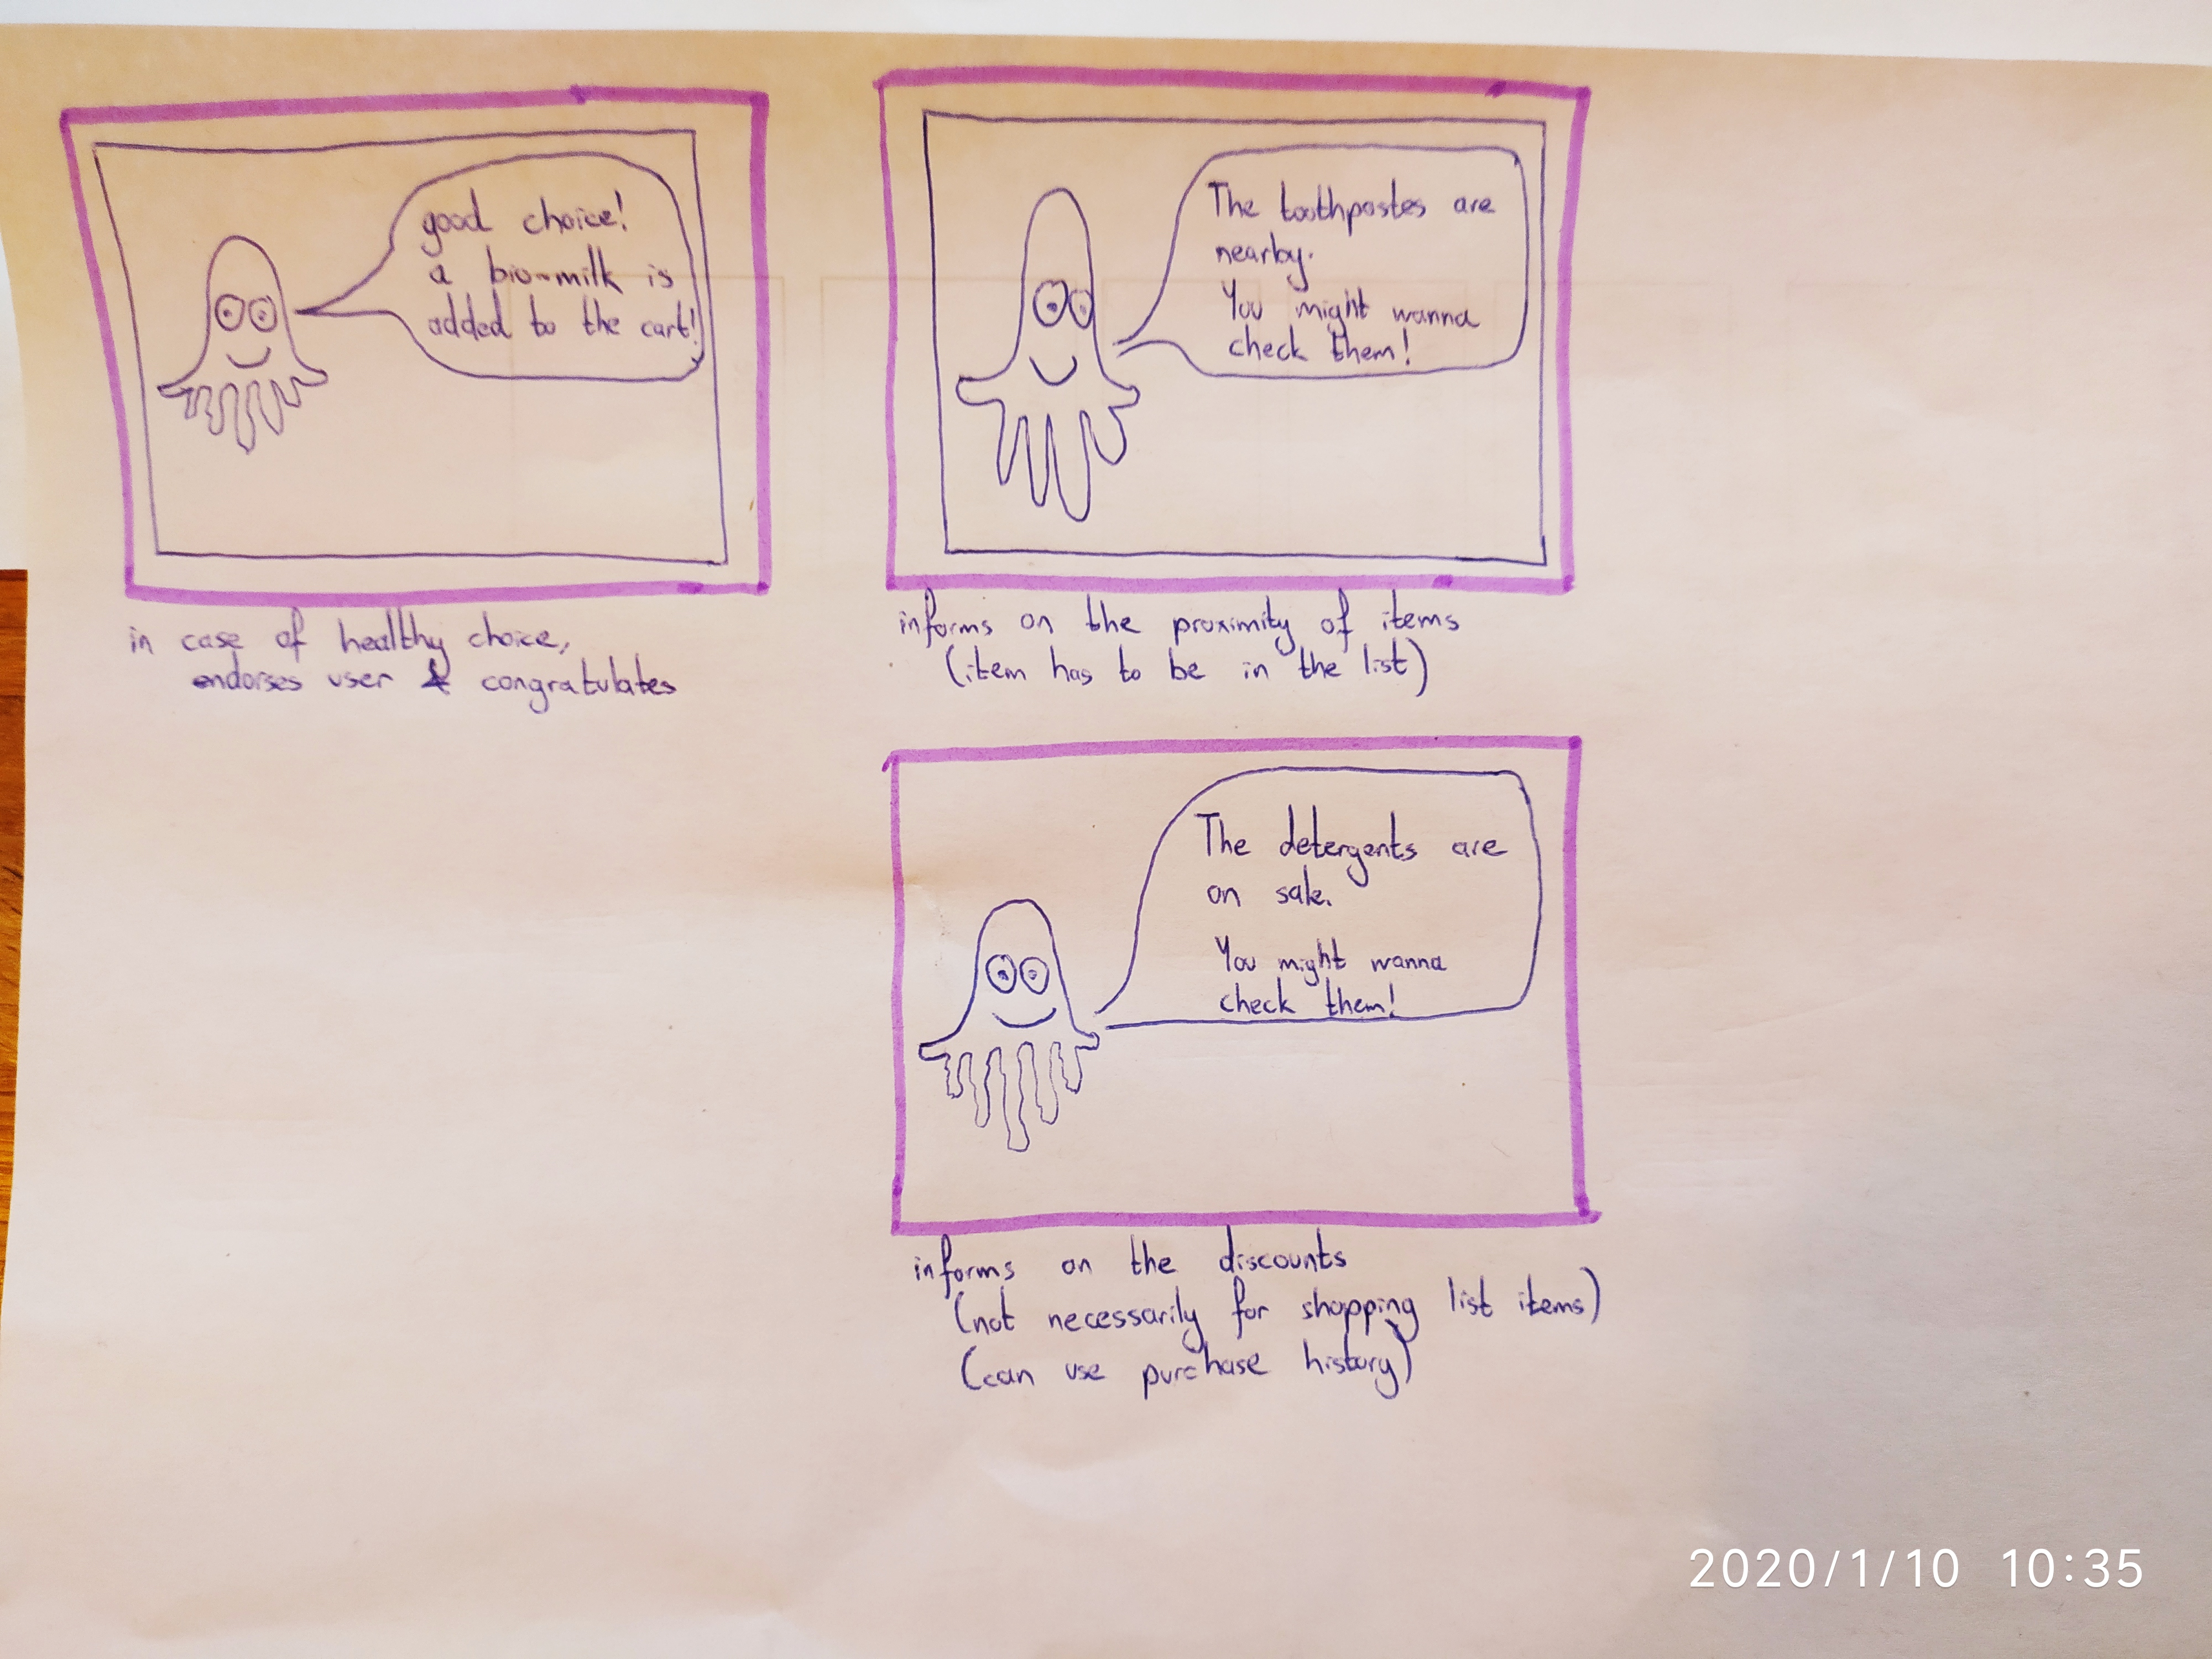
\includegraphics[trim={0em 25em 0em 0em}, clip, width=0.9\textwidth]{images/s1/sb2.jpg}
\end{figure}

\begin{figure}[H]
	\centering
	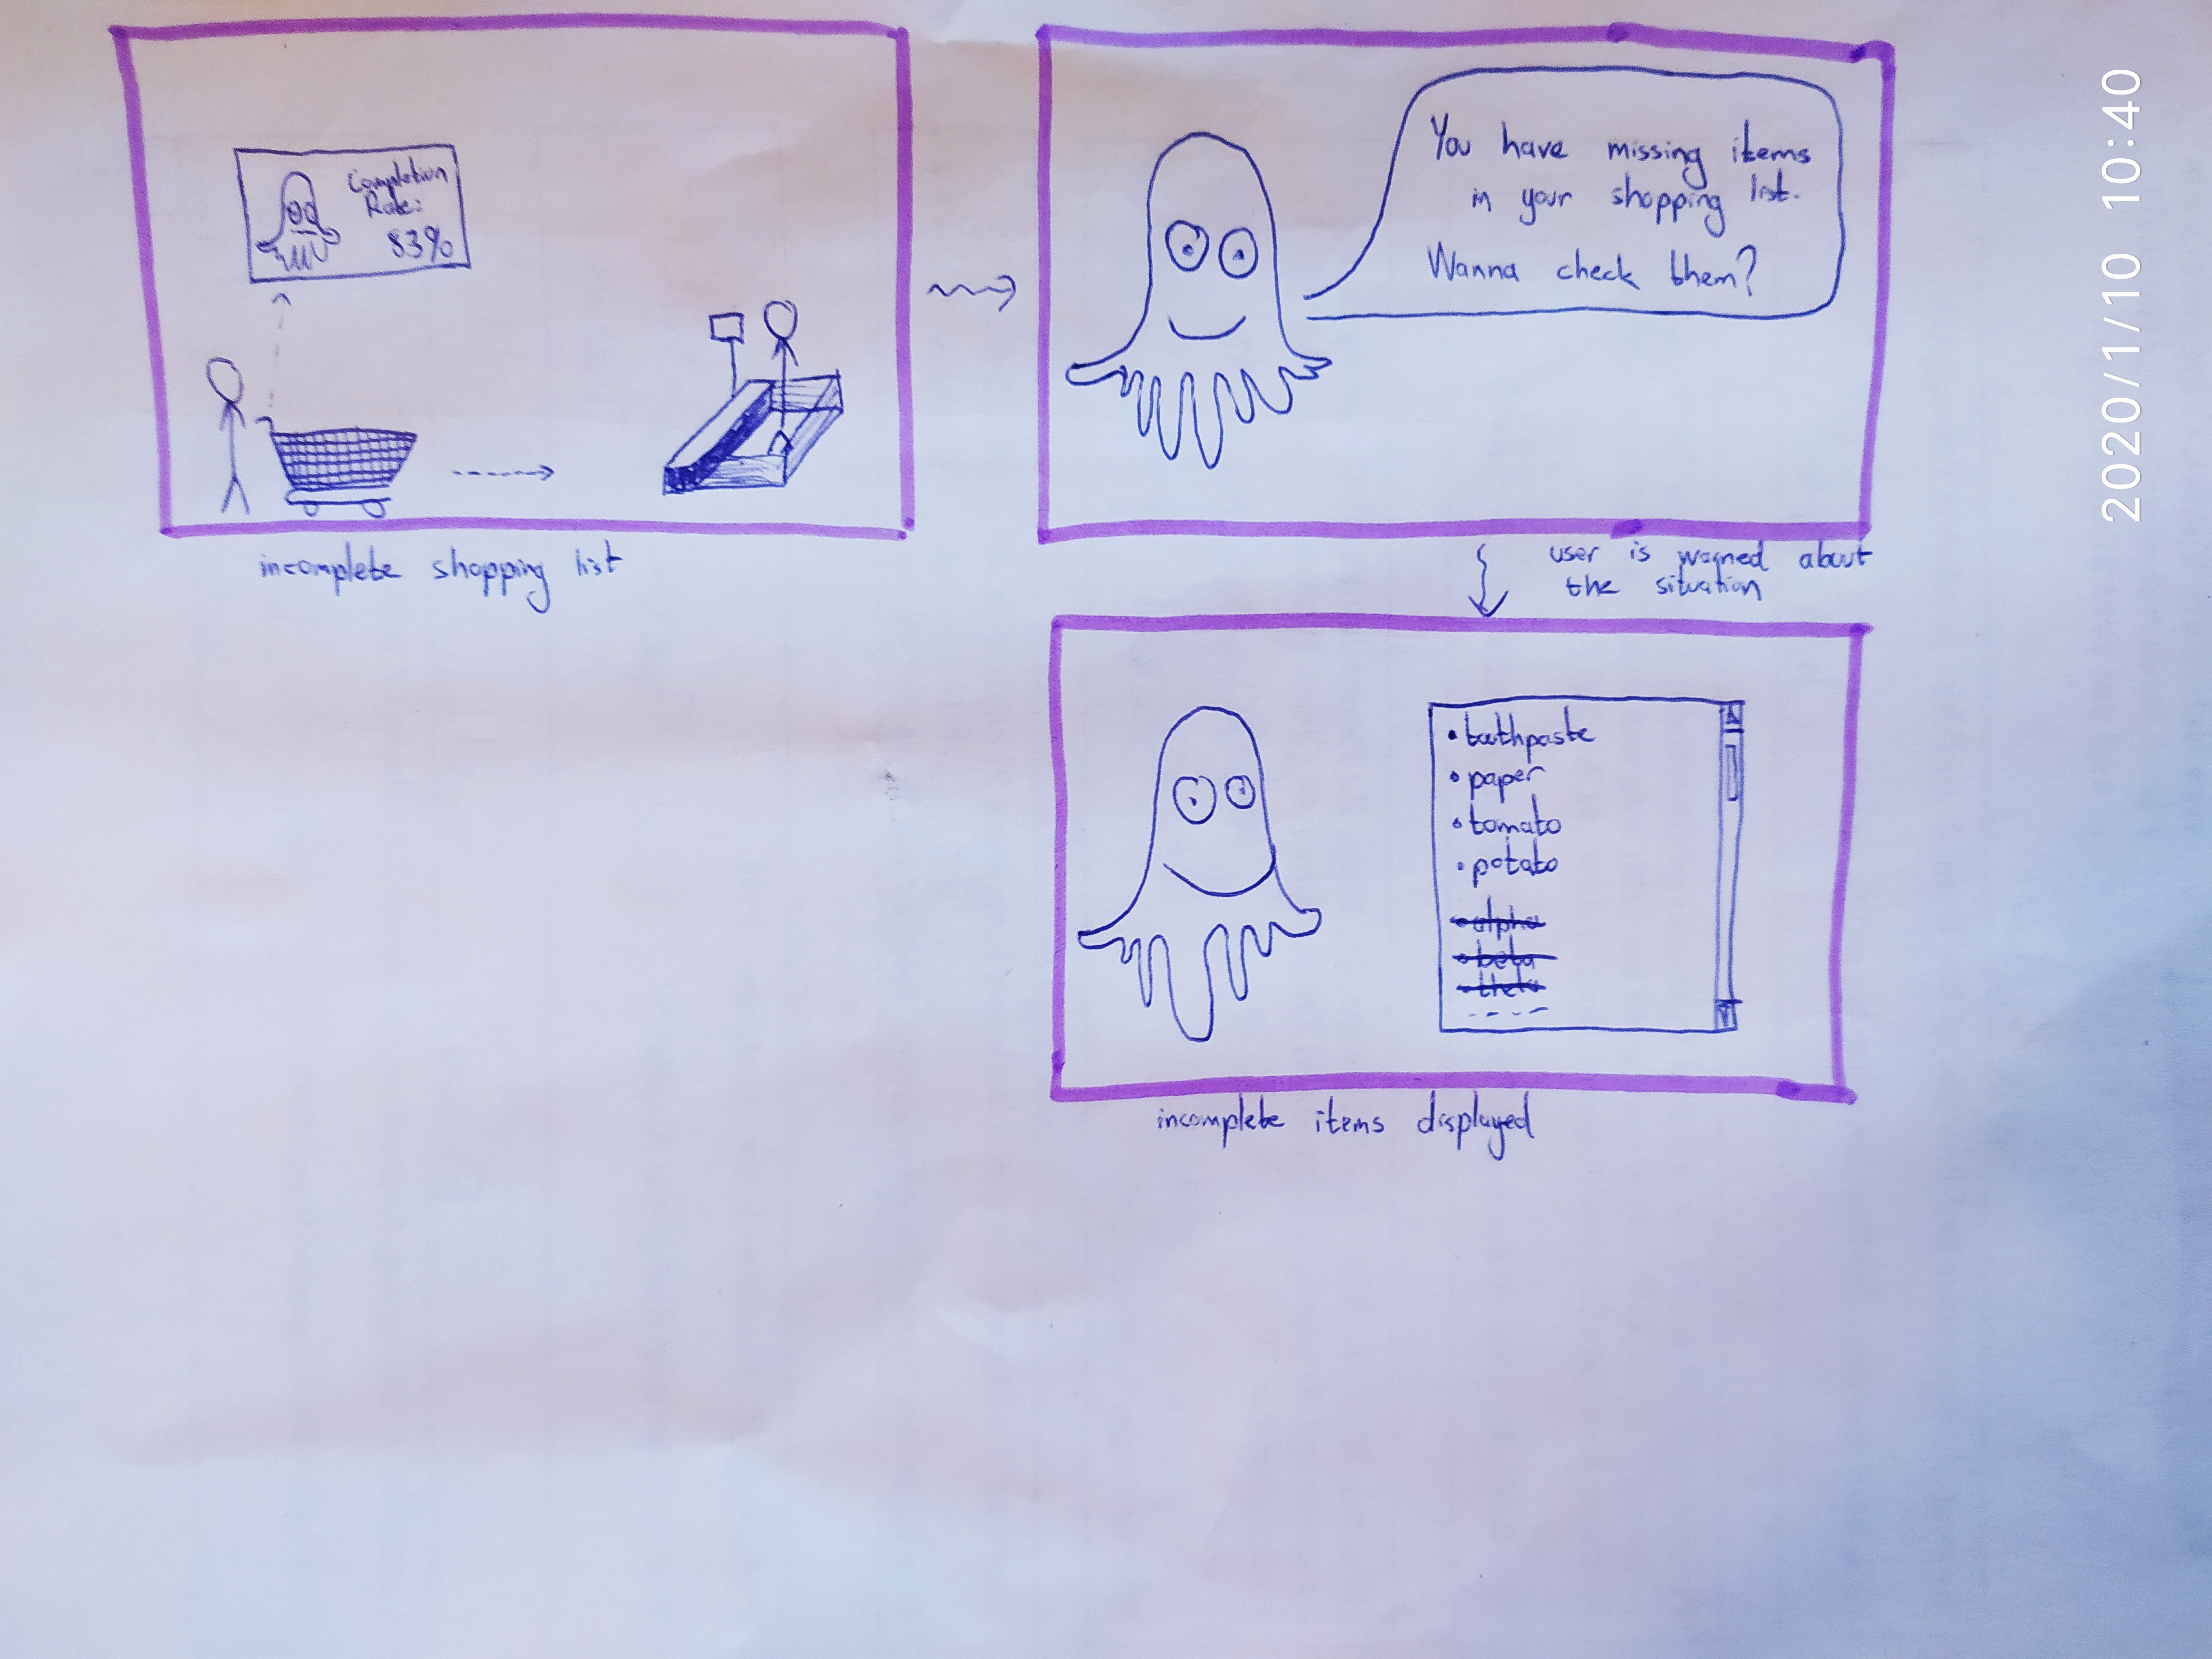
\includegraphics[trim={0em 60em 0em 0em}, clip, width=0.9\textwidth]{images/s1/sb3.jpg}
\end{figure}

\subsection{Core Activities of this Solution}

\begin{itemize}
	\item synchronization of a shopping list, from a smartphone to the tablet attached to the handle of a shopping cart
	
%	\item barcode scanning
	
	\item companion communicating with the user about the general shopping issues (discounts, completed percentage of a shopping list)
\end{itemize}

\subsection{The Reason for Prototype Selection}

We picked paper prototype, as we are designing a tablet application. The use of this product would be heavily depending on the interaction of a user with the graphical user interface of the application.\\

Although we did not glue those papers together, this prototype is designed with flipbook prototypes in mind, and will be adjusted to be displayed under a cardboard which resembles a tablet.

\subsection{Prototyping Process Explained}

We identified the core activities of this solution, as stated above. Based on those identified core activities, we also listed all the possible interactions of a user with the system. Those are:
\begin{itemize}
	\item welcome screen\\
	(\autoref{s1:synch} top)
	
	\item synchronization of shopping list (from smartphone to tablet)\\
	(\autoref{s1:synch} bottom)
	
	\item barcode scanning, and removal of respective items from the list based on what is scanned\\
	(\autoref{s1:barcode} top and bottom)
	
	\item notifications about proximity and discount of products \\
	(\autoref*{s1:offer} top and bottom)
	
	\item incomplete cart notification \\
	(\autoref{s1:percentage})
\end{itemize}

\clearpage
\subsection{Prototype Itself}

\begin{figure}[H]
	\centering
	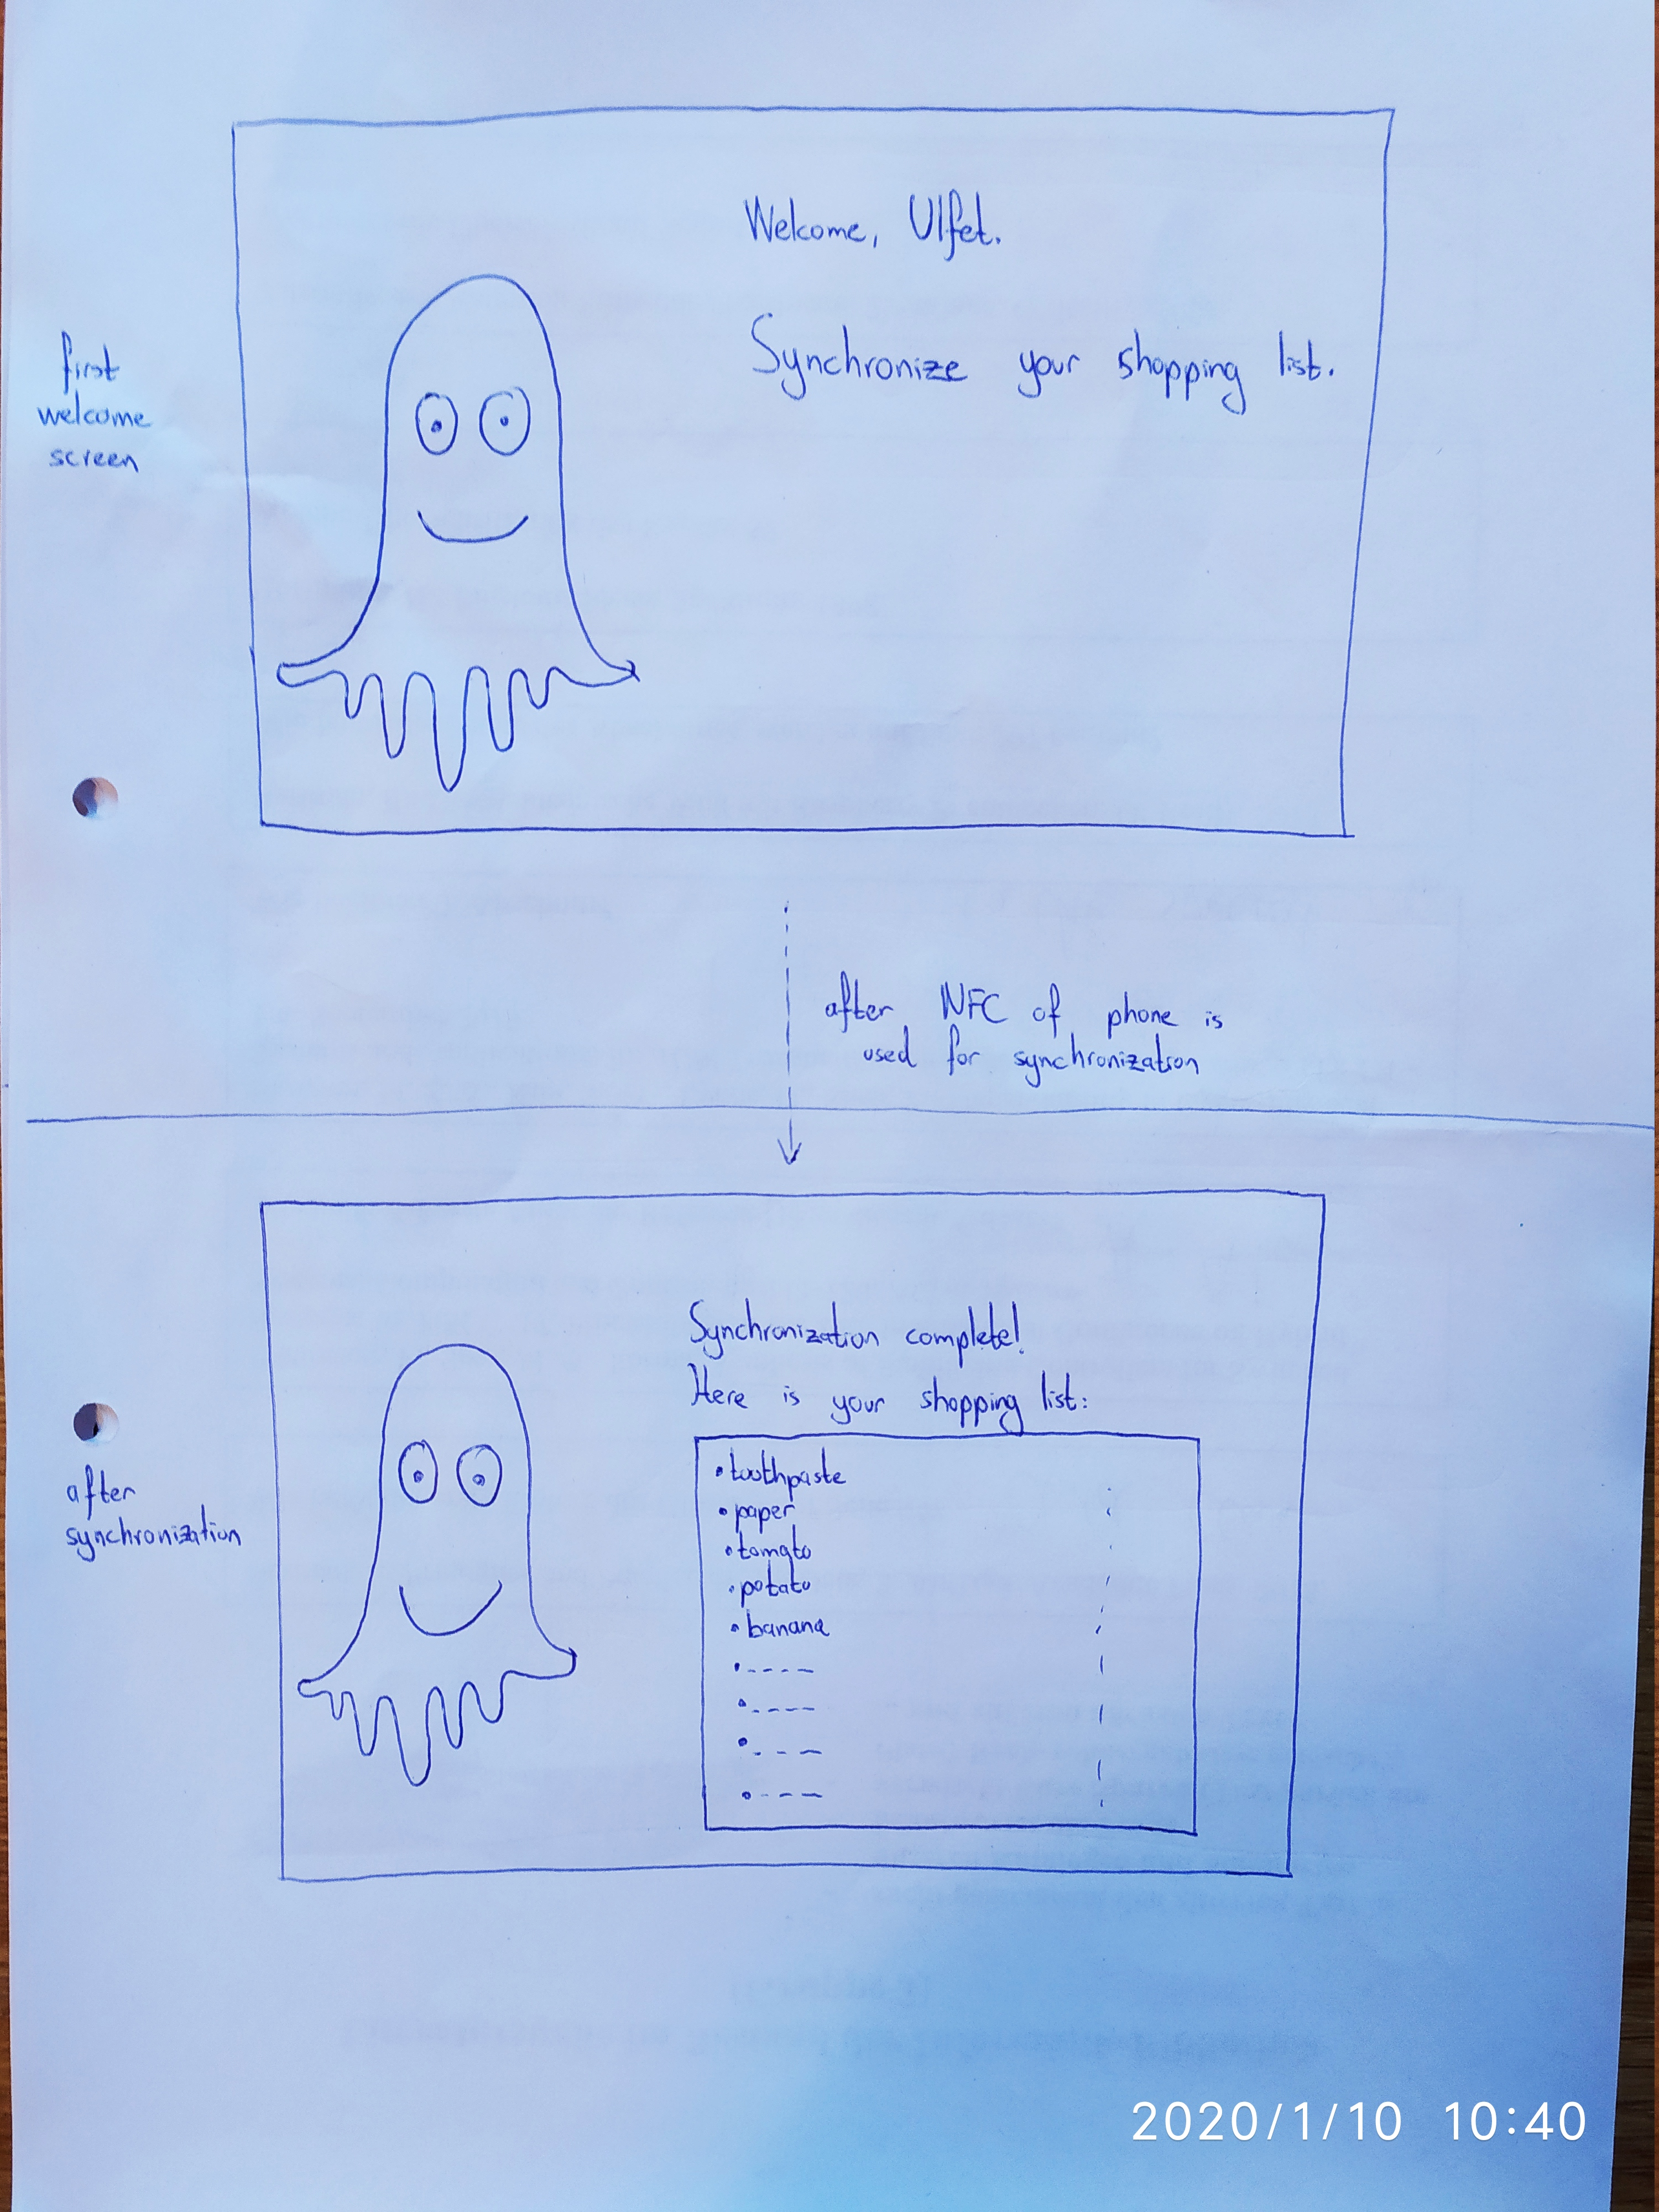
\includegraphics[trim={0em 50em 30em 0em}, clip, width=0.90\textwidth]{images/s1/p1.jpg}
	\caption{Top: The Welcome Screen for Synchronization \& Bottom: after synchronization}
	\label{s1:synch}
\end{figure}

\begin{figure}[H]
	\centering
	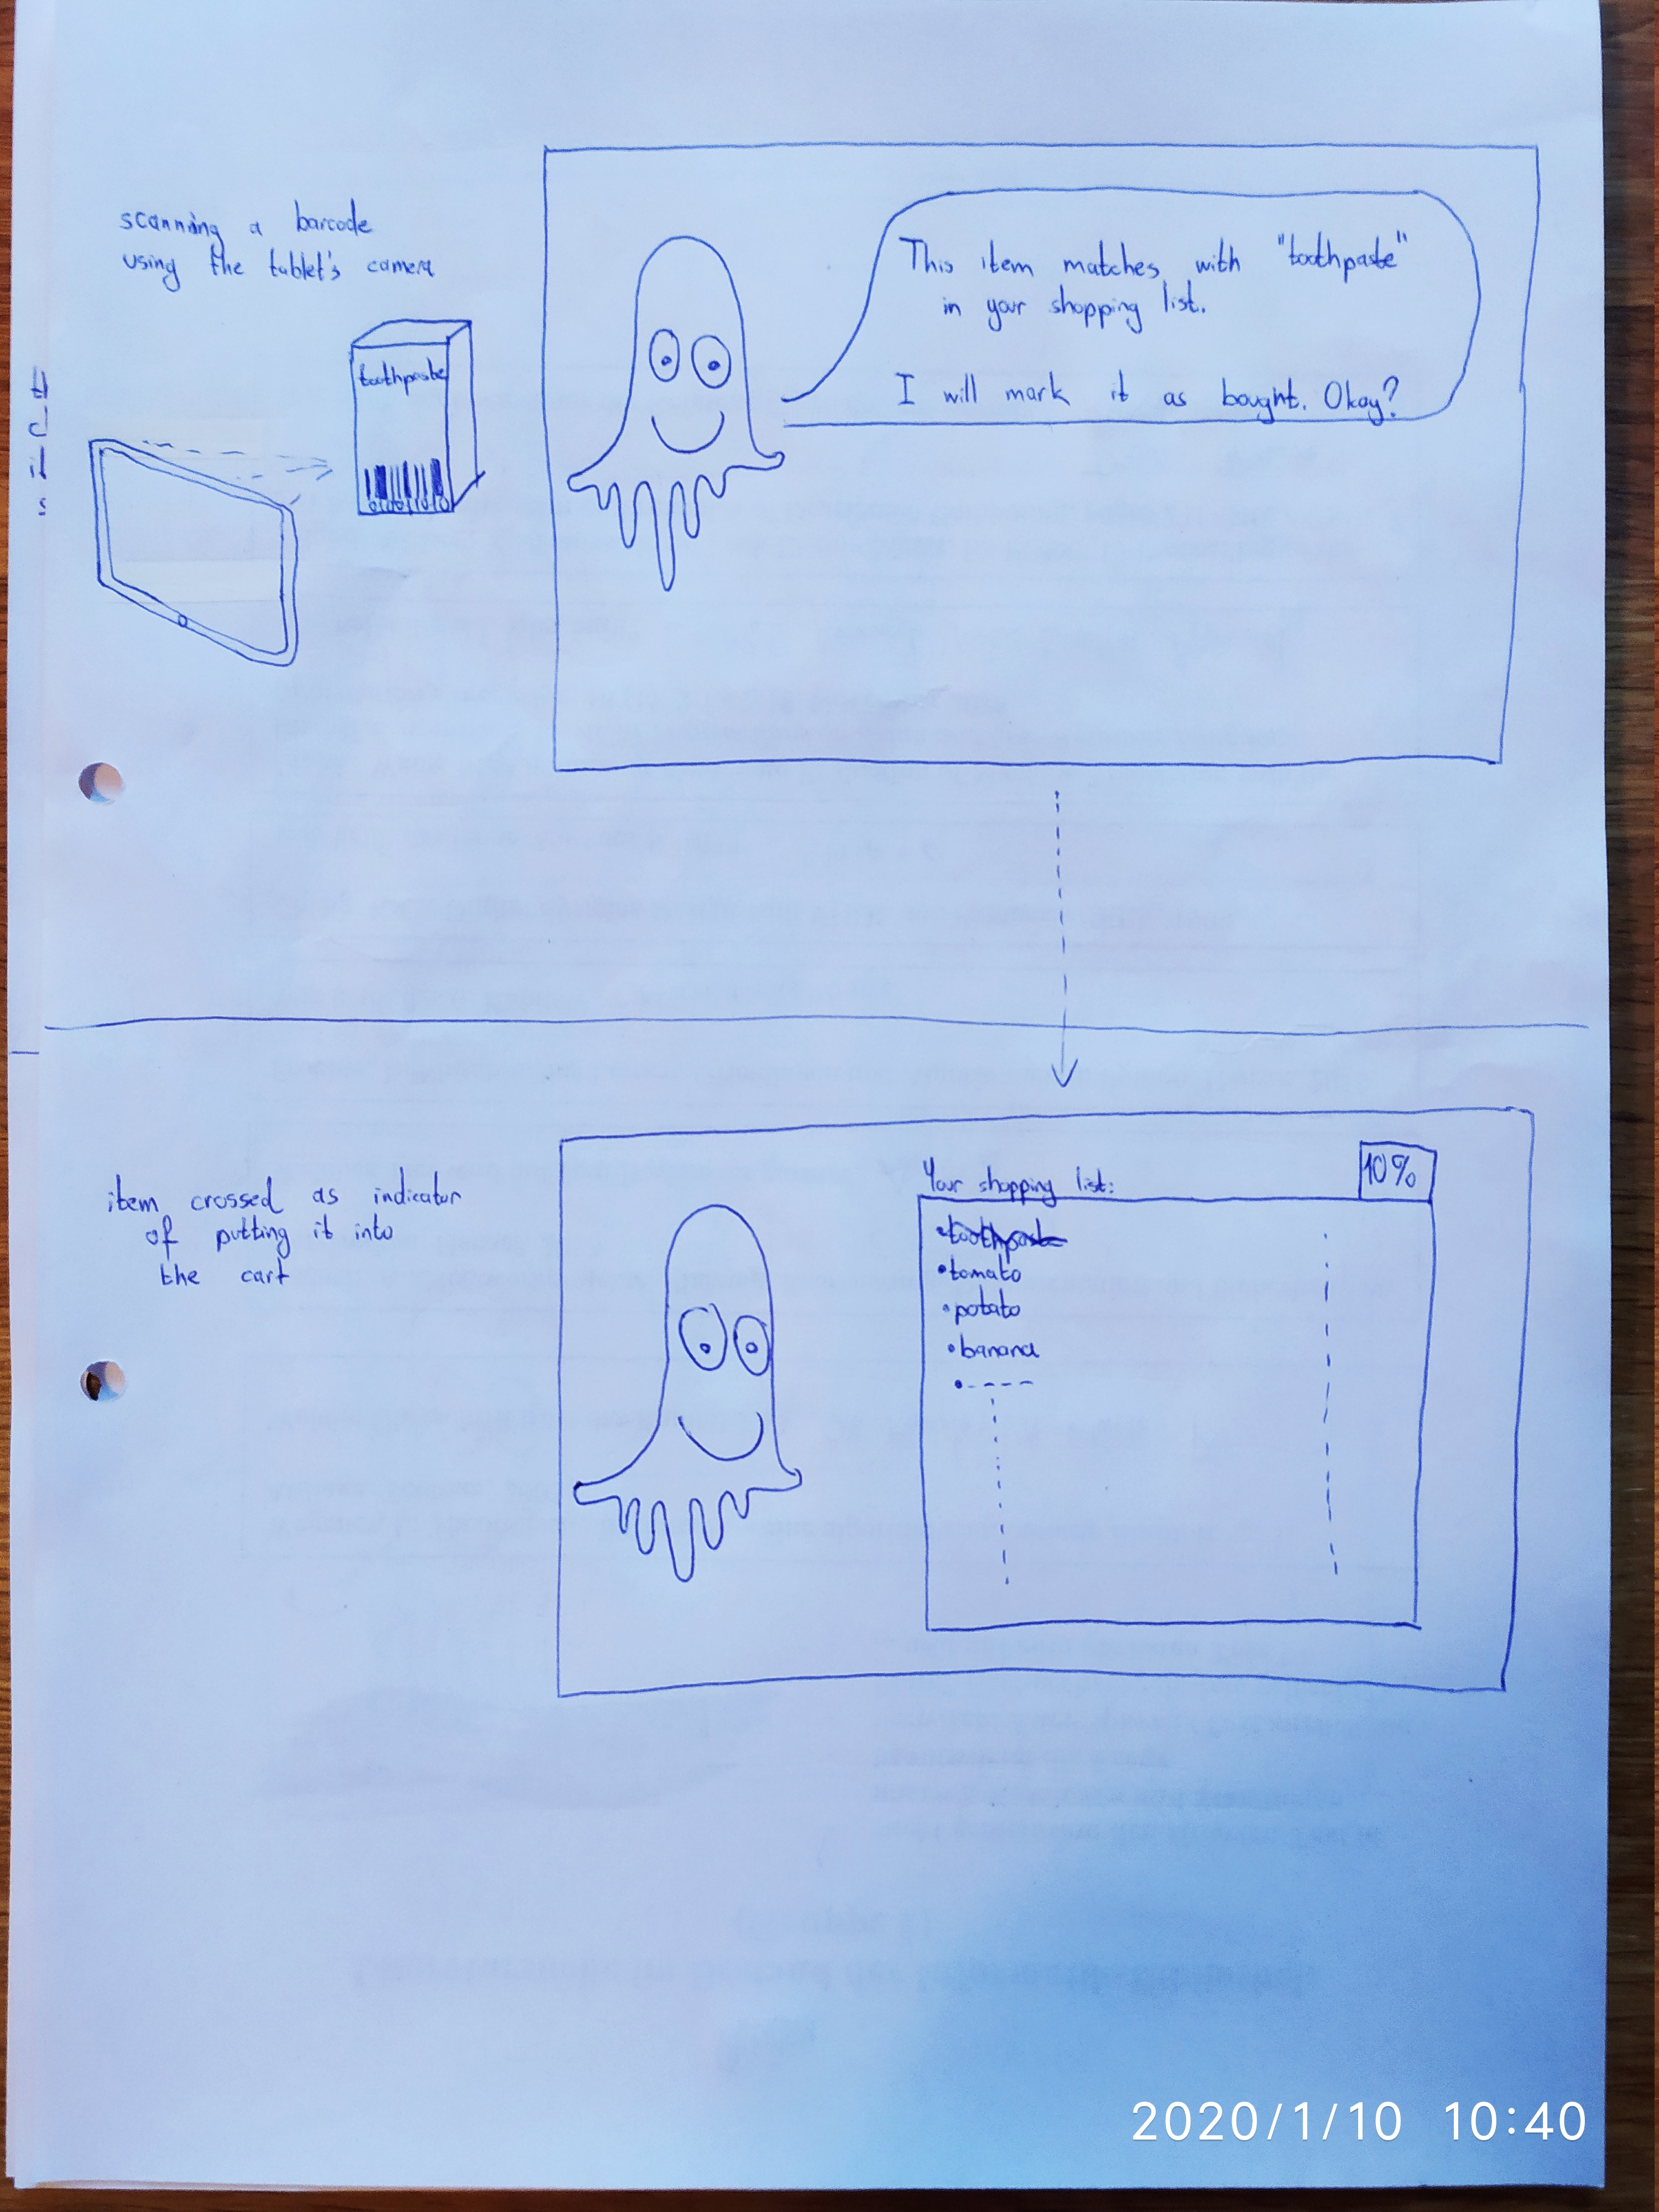
\includegraphics[trim={0em 90em 20em 0em}, clip, width=0.9\textwidth]{images/s1/p2.jpg}
	\caption{Top: Barcode Scanning \& Bottom: Scanned Item Removed from the Shopping List}
	\label{s1:barcode}
\end{figure}

\begin{figure}[H]
	\centering
	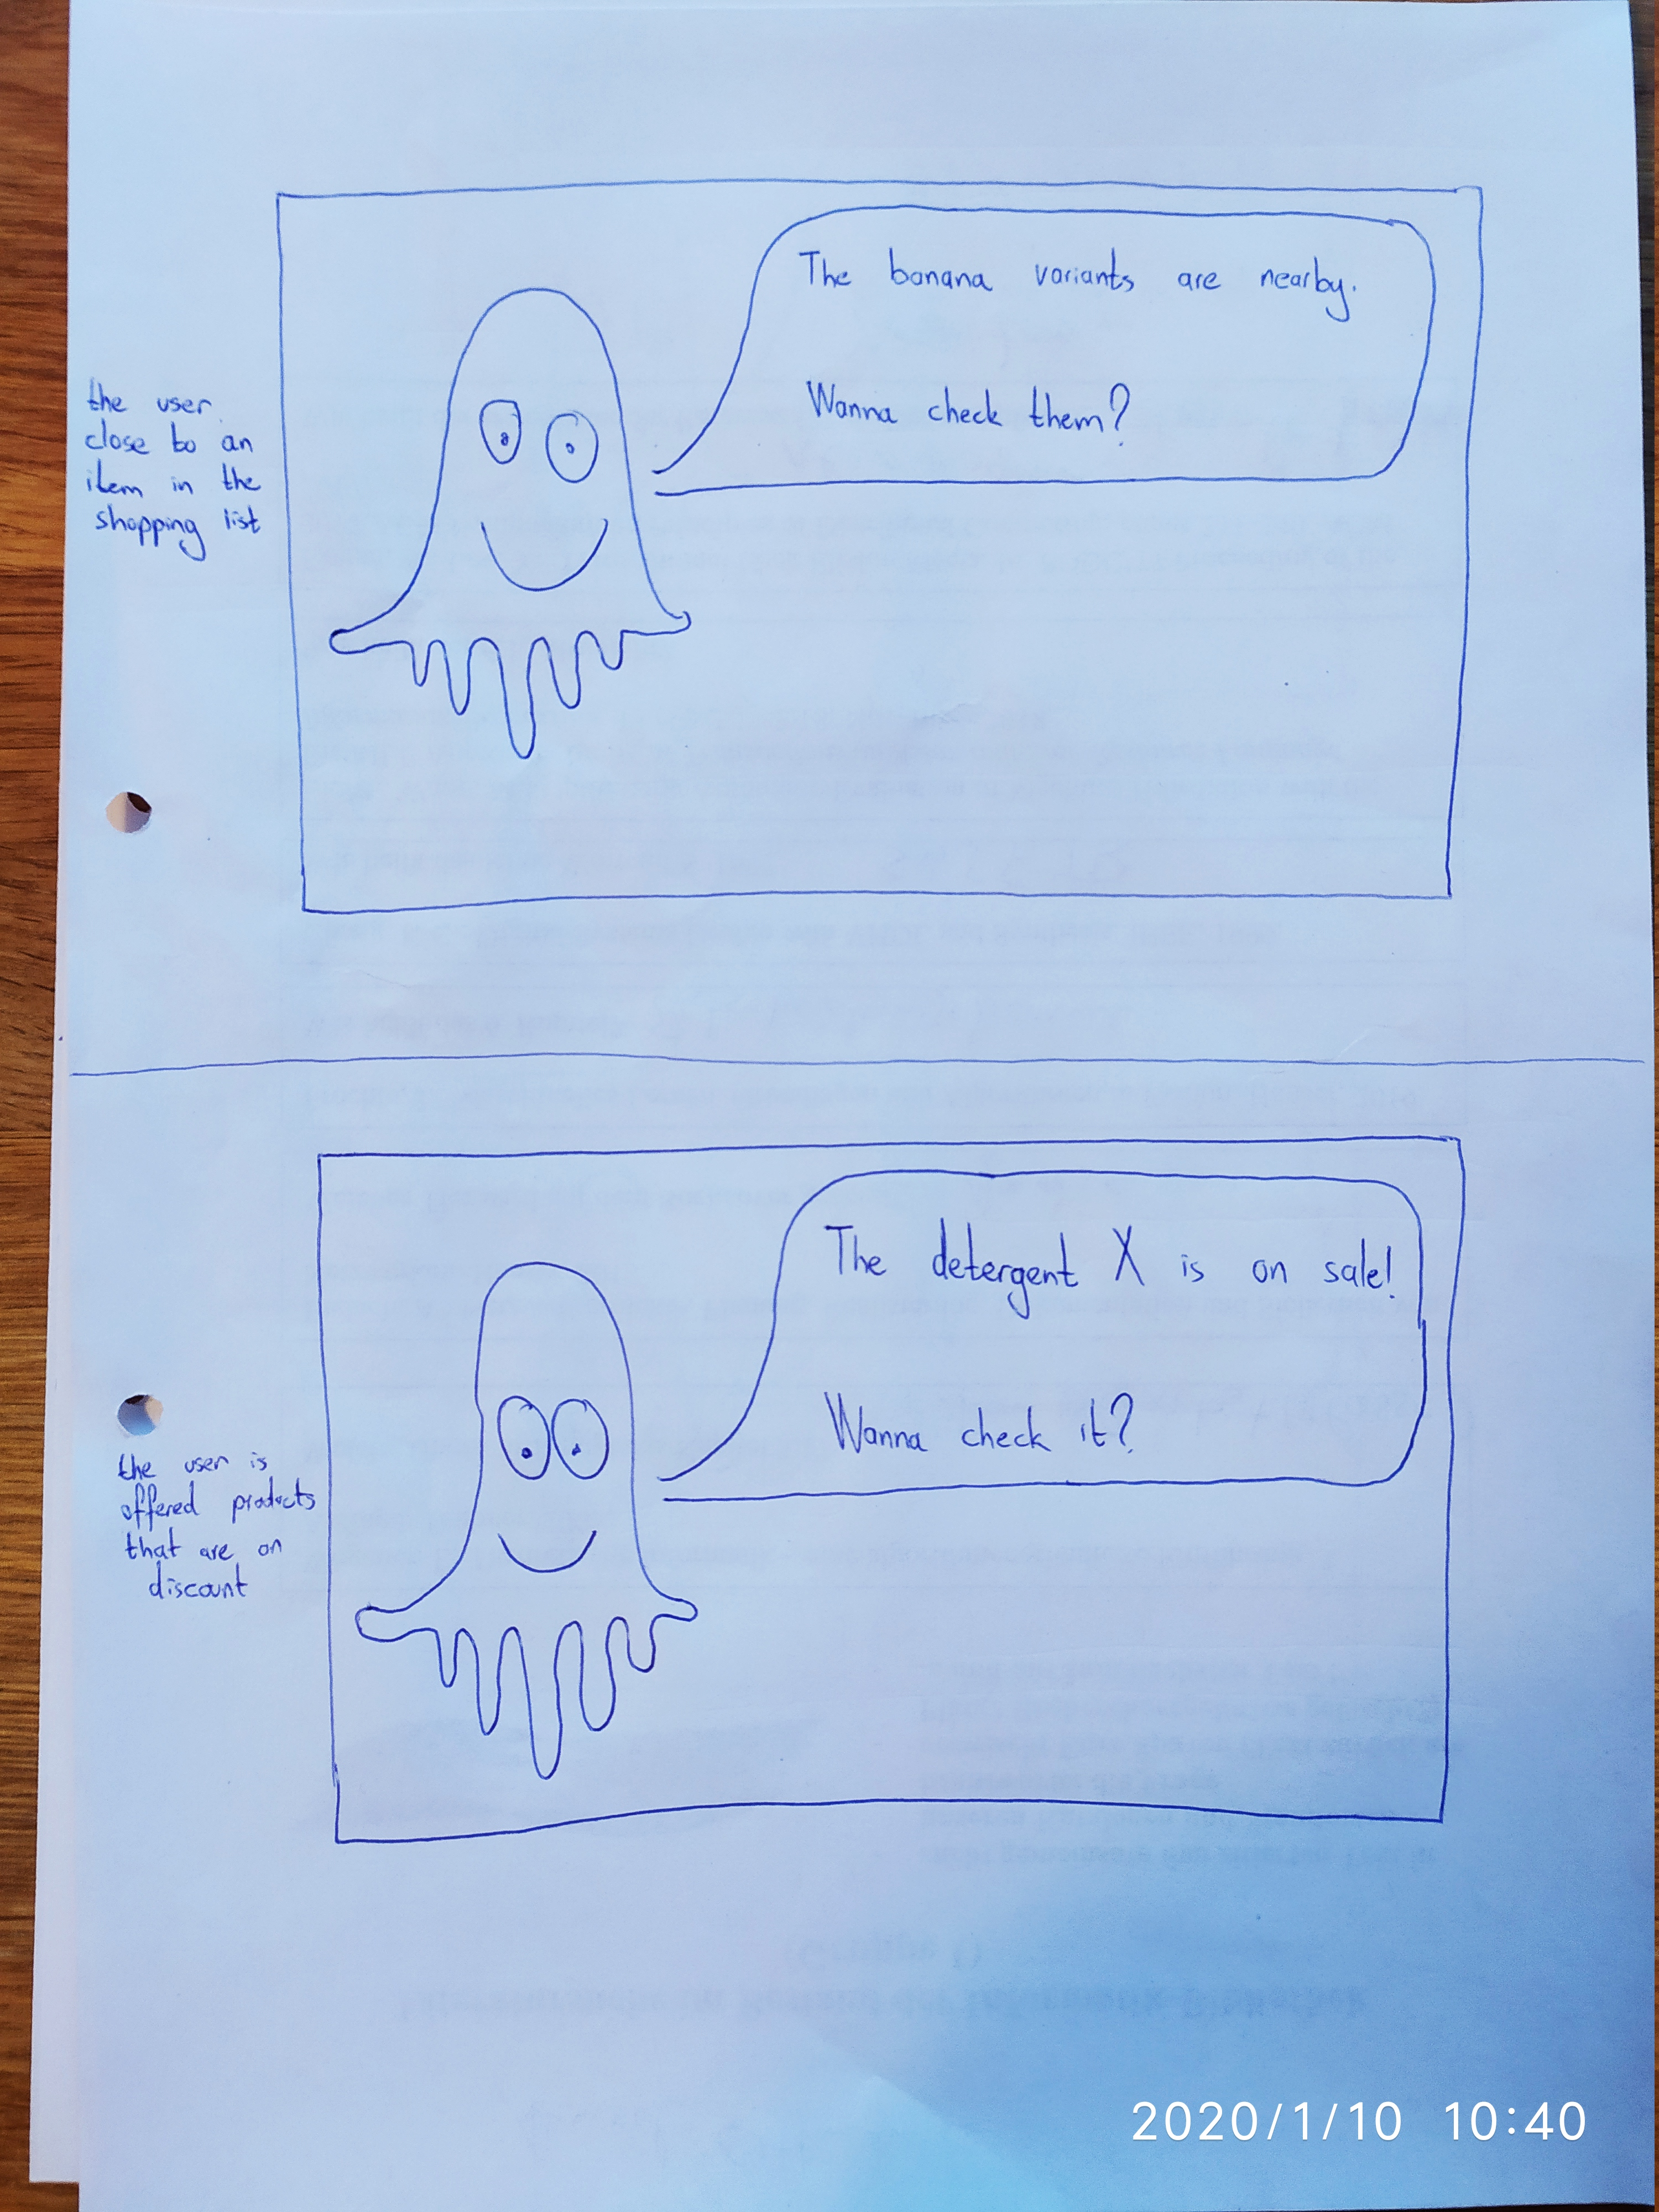
\includegraphics[trim={10em 60em 20em 0em}, clip, width=0.9\textwidth]{images/s1/p3.jpg}
	\caption{Top: Nearby Items Recommended based on Shopping List \& Bottom: Discounted Items are Offered}
	\label{s1:offer}
\end{figure}

\begin{figure}[H]
	\centering
	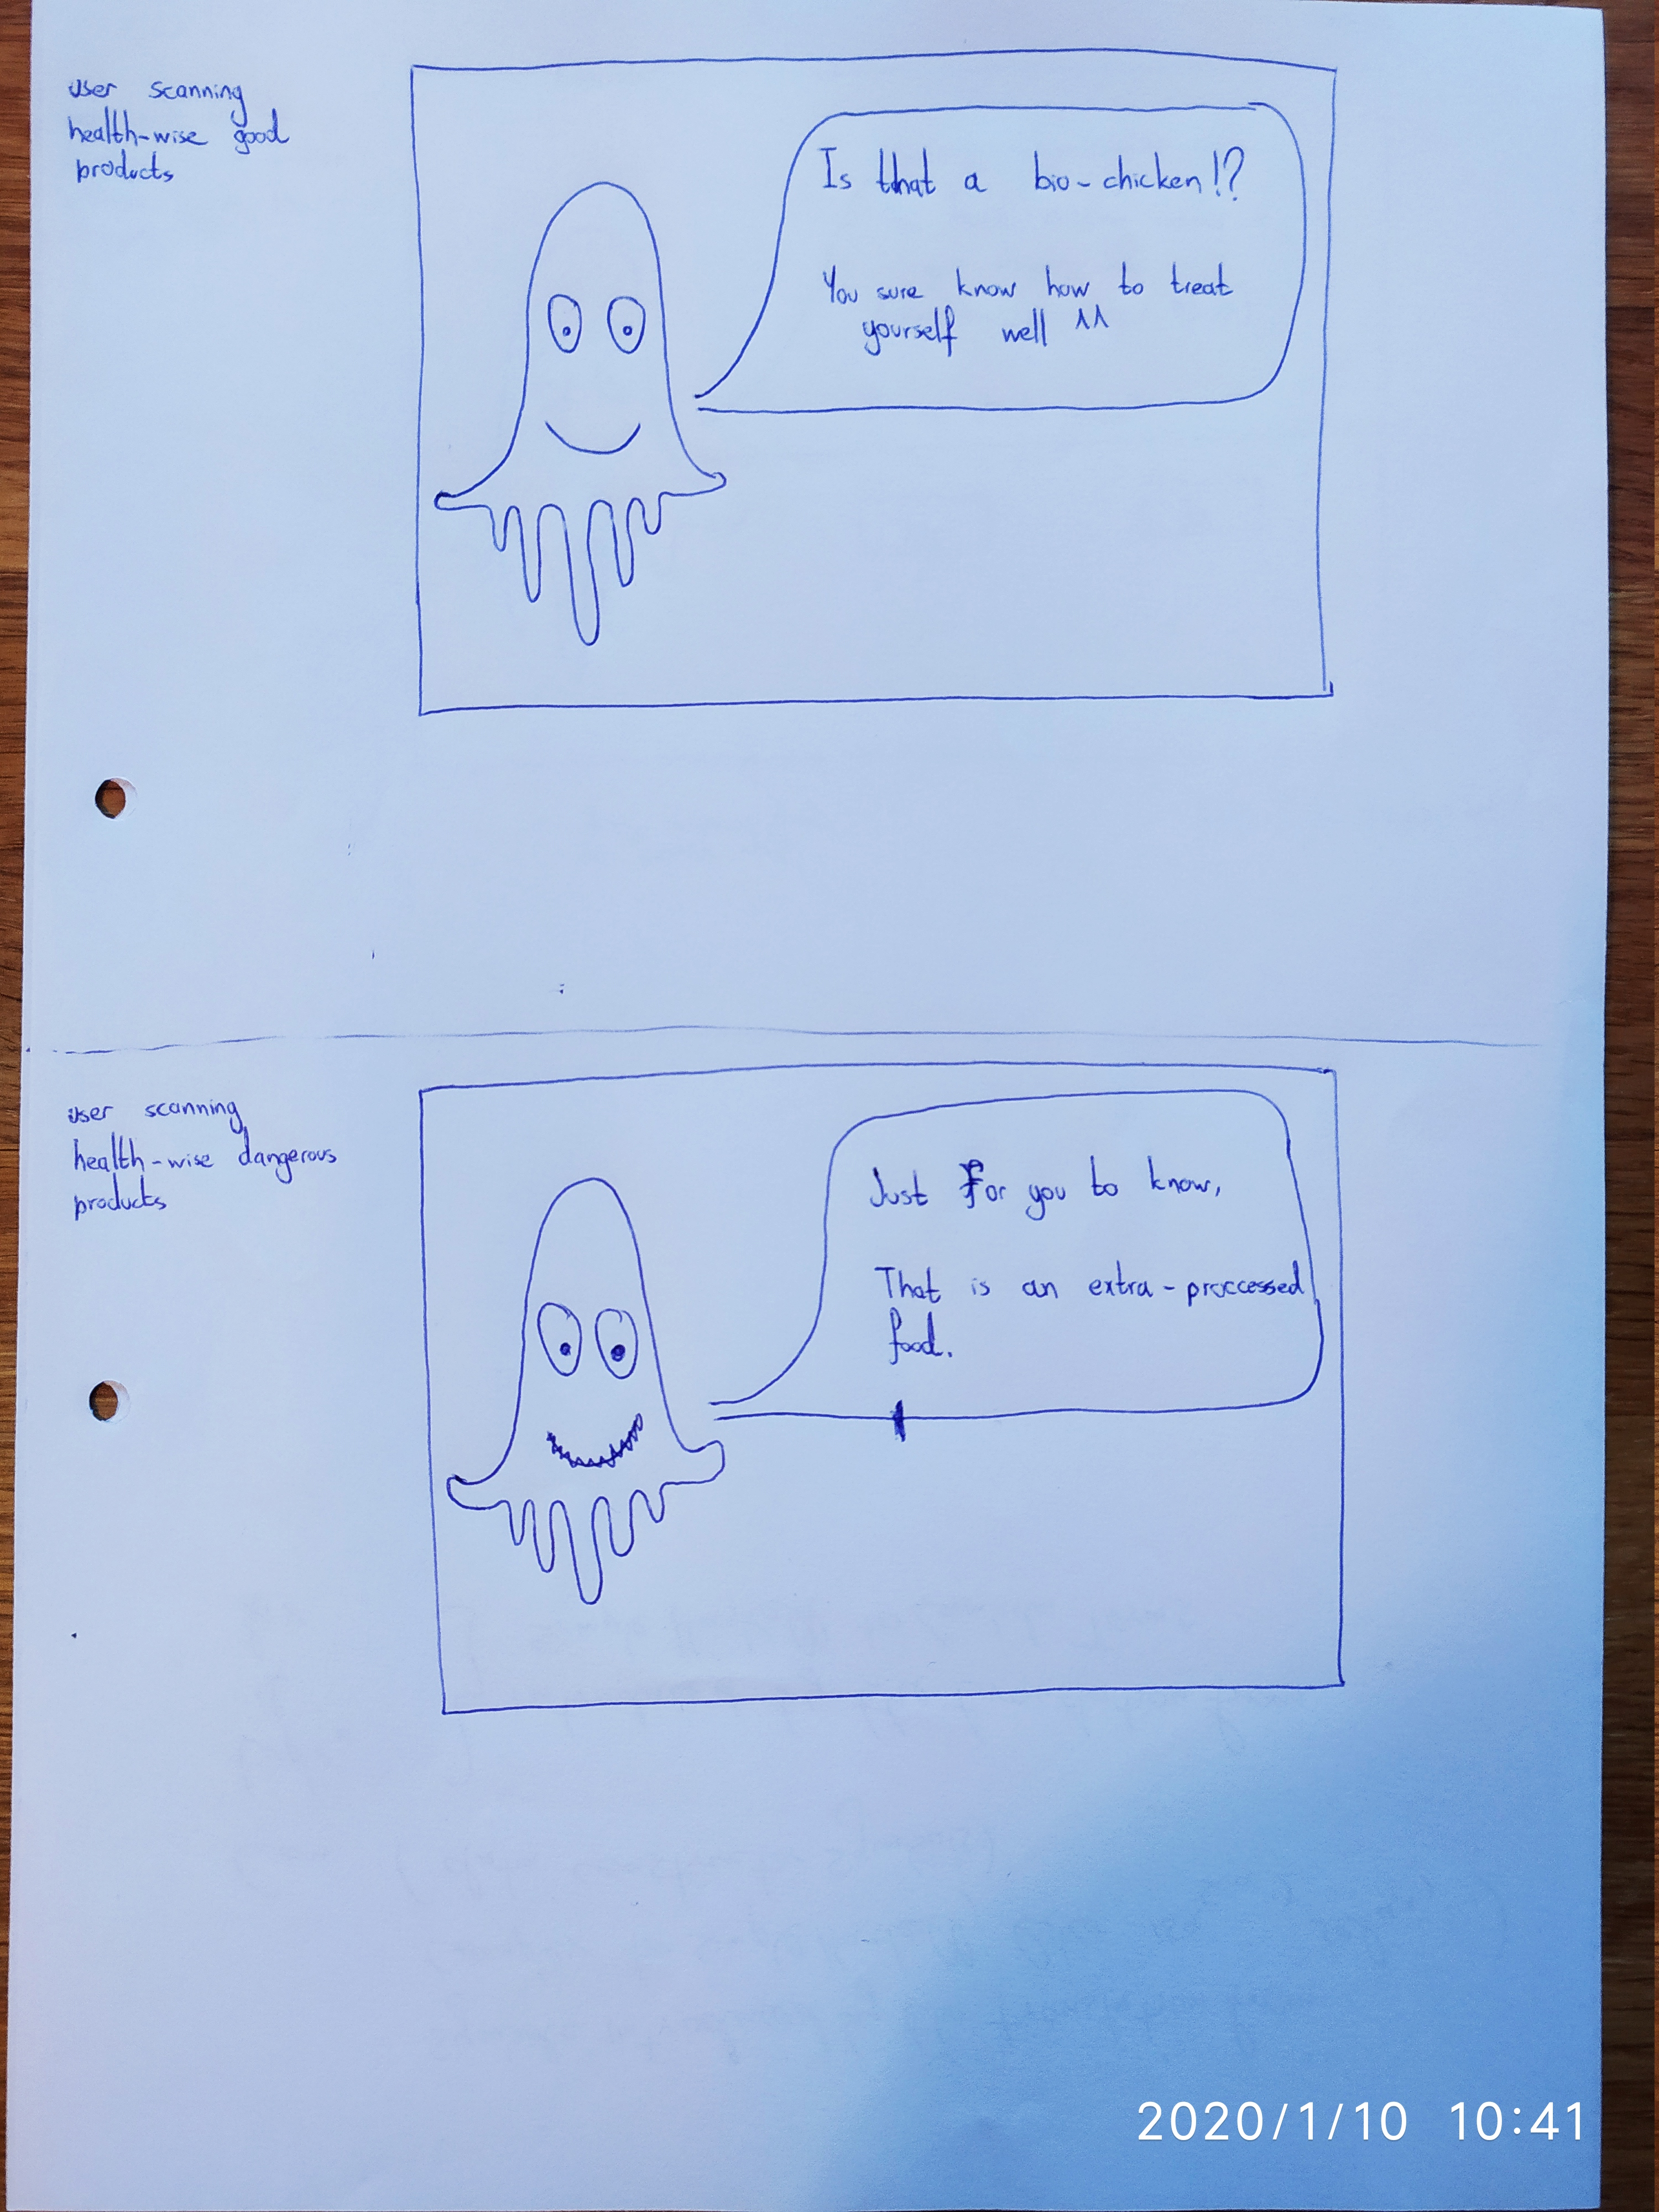
\includegraphics[trim={10em 80em 40em 0em}, clip, width=0.9\textwidth]{images/s1/p4.jpg}
	\caption{User Informed about the Quality of the Product}
	\label{s1:comment}
\end{figure}

\begin{figure}[H]
	\centering
	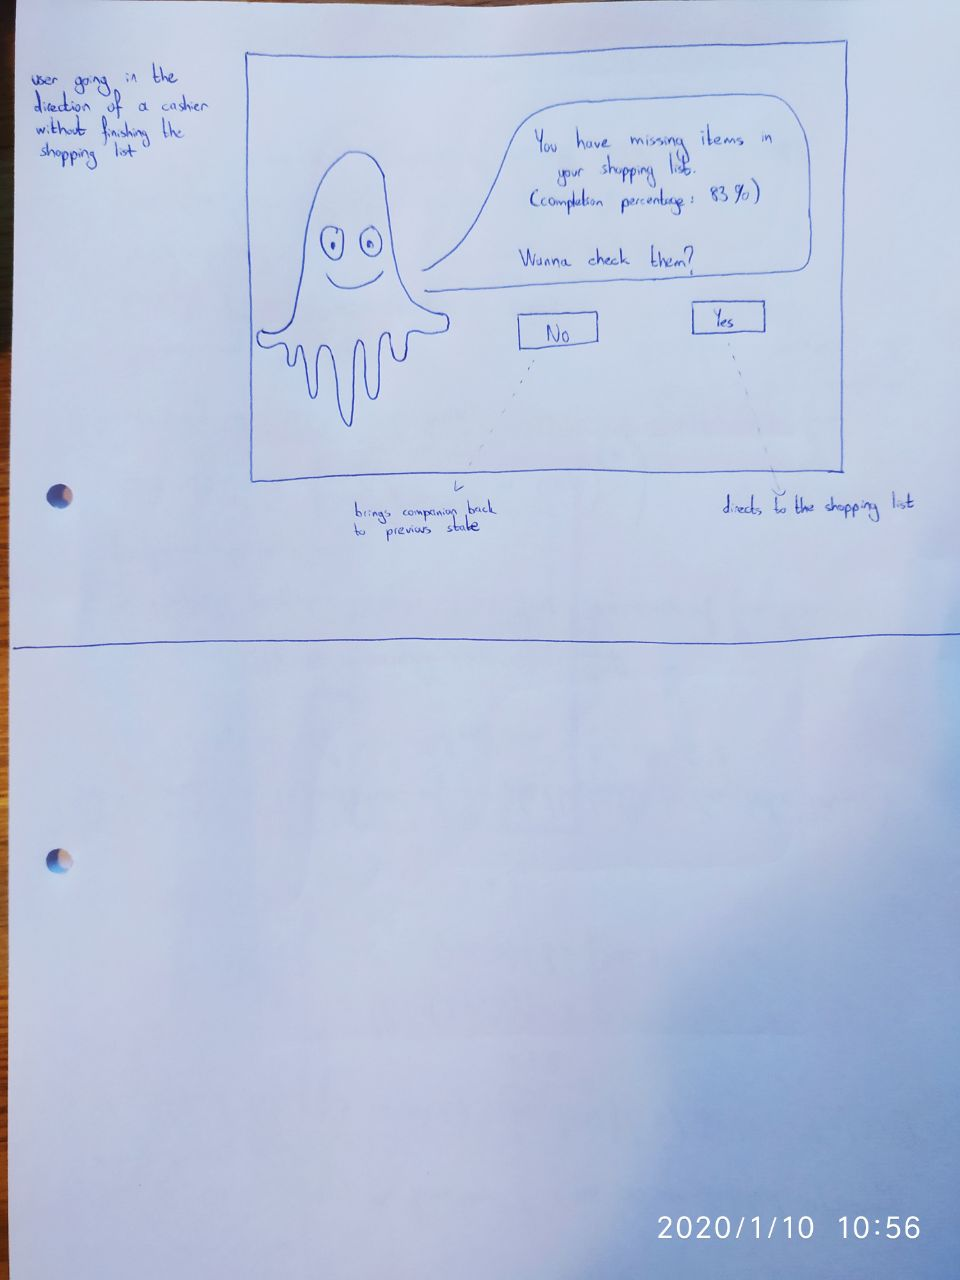
\includegraphics[trim={0em 70em 0em 0em}, clip, width=0.9\textwidth]{images/s1/p5.jpg}
	\caption{The Shopping List Completion Percentage: the user is notified about it in case it is not completed}
	\label{s1:percentage}
\end{figure}